	\documentclass[oneside,senior,etd]{BYUPhysForDegree}

\usepackage[utf8]{inputenc}
\usepackage{rotating} 
\usepackage{indentfirst} 
\usepackage{url}

\usepackage[russian]{babel}
\usepackage{amsfonts} % Пакеты для математических символов и теорем
\usepackage{amstext}
\usepackage{amssymb}
\usepackage{amsthm}
\usepackage{graphicx} % Пакеты для вставки графики
\usepackage{subfig}
\usepackage{color}
\usepackage[unicode]{hyperref}
\usepackage[nottoc]{tocbibind} % Для того, чтобы список литературы отображался в оглавлении
\usepackage{algorithmic} % Для записи алгоритмов в псевдокоде
\usepackage{algorithm}
\usepackage{verbatim} % Для вставок заранее подготовленного текста в режиме as-is
\usepackage{listings}

\usepackage{commath}
\newcommand\Tau{\mathcal{T}}
\newcommand{\R}{\mathbb{R}}
\usepackage{color}
\usepackage[colorinlistoftodos, prependcaption]{todonotes}
\usepackage{multirow}
\newcommand*{\MyIndent}{\hspace*{0.2cm}}%

\Chair{Кафедра Системного Программирования}
\Lab{~}
\Year{2021}
  \Month{Май}
  \City{Москва}
  \AuthorText{Автор}
  \Author{Лазарев Владимир Александрович}
  \AuthorEng{}
  \AcadGroup{528}
  % Если вы не Пупкин Василий Иванович, то скопируйте себе этот проект через меню и уже потом правьте
  \TitleTop{Исследование методов OSINT для}
  %\TitleMiddle{}
  \TitleBottom{поиска информации о человеке} % leave empty if you don't need it
%   \TitleTopEng{Research and development of machine learning methods}
%   \TitleBottomEng{} % leave empty if you don't need it  
  \docname{Курсовая работа}
  %\docname{Выпускная квалификационная работа}
  %\docname{Магистерская диссертация}
  \Advisor{Турдаков Денис Юрьевич}  
  \AdvisorDegree{к.ф.-м.н.}
%   \Consultant{Варламов Максим}
  \Consultant{Яцков Александр Константинович}
  \ConsultantDegree{}
  
\Abstract{\parДанная работа посвящена исследованию и разработке методов OSINT для поиска информации о человеке. 
 Данная курсовая содержит описание реализованных методологий и повествует о созданных приемах извлечения информации. 
 \parВ ходе работы были изучены и представлены существующие различные методы как по способу взаимодействия с сервисами: 
  извлечение данных с web-страницы и посредством скрытого или открытого api; 
  так и по типу сервиса: поисковый агрегатор и социальные сети.}
\AbstractEng{Abstract}


%%%% DON'T change this. It is here because .sty does not support cyrillic cp properly %%%%
\University{Московский государственный университет имени М.В.Ломоносова}
\Faculty{Факультет вычислительной математики и кибернетики}
\GrText{гр.}
\AdvisorText{Научный руководитель}
\ConsultantText{Научный консультант}
\AbstractText{Аннотация}

\begin{document}
\fixmargins
\makepreliminarypages

\oneandhalfspace

\tableofcontents

\section{Введение}
\label{sec:Chapter0} \index{Chapter0}

\todo[inline]{Если вы не Пупкин Василий Иванович, то скопируйте себе этот проект через меню и уже потом правьте}
\todo[inline]{В этой части надо описать предметную область, задачу из которой вы будете решать, объяснить её актуальность (почему надо что-то делать сейчас?).
Здесь же стоит ввести определения понятий, которые вам понадобятся в постановке задачи.} % Введение
\section{Постановка задачи}
\label{sec:Chapter1} \index{Chapter1}
\todo[inline]{Здесь надо максимально формально описать суть задачи, которую потребуется решить, так, чтобы можно было потом понять, в какой степени полученное в результате работы решение ей соответствует. Текст главы должен быть написан в стиле технического задания, т.е. содержать как описание задачи, так и некоторый набор требований к решению} % Постановка задачи
\section{Обзор существующих решений}
\label{sec:Chapter2} \index{Chapter2}
\subsection{Поиск данных в поисковых сервисах}
\subsubsection{Бедолага1}
\subsubsection{Бедолага2}
\subsection{Поиск данных в социальных сетях}
\subsubsection{Бедолага3}
\subsubsection{Бедолага4}
 % Обзор существующих решений
\section{Исследование и построение решения задачи}
\label{sec:Chapter3} \index{Chapter3}
С целью исследования и разработки своих собственных OSINT методов сбора информации о человеке с помощью поисковых сервисов и 
социальных сетей предстоит решить следующие задачи:
\begin{itemize}
    \item поисковые сервисы:
    \begin{enumerate}
        \item Определить структуру поискового сайта. В качестве таких сайтов возьмем следующие ресурсы:
        \begin{itemize}
            \item DuckDuckGo;
            \item Google;
            \item Yandex;
            \item Yahoo.
        \end{itemize}
        \item Извлечение найденных ссылок по заданному ключевому слову.
        \item Сбор информации с сайтов по отобранным ссылкам.
        \item Для случая с Google попробовать Google Search API: определить шаблон GET-запроса, структуру возвращаемых данных.
    \end{enumerate}
    \item социальные сети:
    \begin{enumerate}
        \item Определить структуру сайта социальной сети. Будем работать над социальной сетью LinkedIn.
        \item Реализовать поиск и сбор данных пользователей и организаций посредством веб-краулинга сайта.
        \item Реализовать сбор данных пользователей и организаций посредством закрытого API LinkedIn. Для этого потребуется:
        \begin{itemize}
            \item реализовать вход систему через закрытое API посредством GET и POST запросов;
            \item определить шаблон GET-запроса для получения данных по указанным ключевым словам, структуру возвращаемых данных.
        \end{itemize}
    \end{enumerate}
    \item реализовать все указанные выше подзадачи в систему сбора данных. 
\end{itemize}
 % Исследование и построение решения задачи
\section{Описание практической части}
\label{sec:Chapter4} \index{Chapter4}
\subsection{Описание выбранного инструментария}
Работа была написана на языке Python, основной фреймворк для сбора данных -- Scrapy, так как эта библиотека позволяет
гибко настраивать параметры запросов, их обработку, генерацию cookie-файлов, поддерживает множественные подключения к ресурсы, 
асинхронно собирает данные \cite{scrapyBook}. В качестве базы данных
выступает MongoDB, поскольку она хранит данные в формате JSON-подобных документов \cite{mongoDBBook}. 

\par
Поскольку поиск в поисковых сервисах и поиск в социальной сети LinkedIn отличается по концепции и настройке пауков Scrapy, то
они были выделены в 2 различных проекта.

\subsubsection{Архитектура работы сборщиков в поисковых сервисах}
\par
Диаграмма классов приведена на рис. 7.

\begin{figure}[H]
    \center{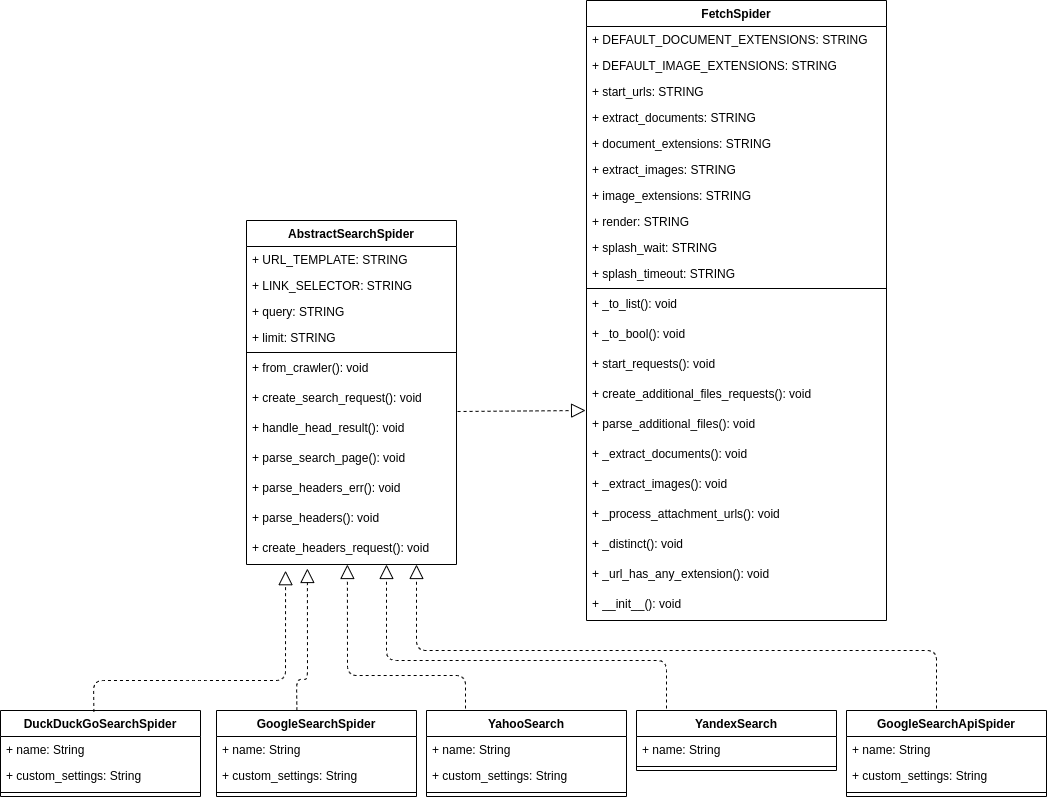
\includegraphics[height=10cm,keepaspectratio]{pictures/SearchNews.png}}
    \caption{Диаграмма классов сборщик в поисковых сервисах.}
    \label{ris:image}
\end{figure}

Система включает следующие 9 классов:
\begin{itemize}
    \item Сборщики данных:
    \begin{itemize}
        \item FetchSpider -- позволяет собирать все документы, изображения и html-код страницы;  
        \item AbstractSearchSpider -- содержит общие метода генерации запросов, обхода страниц и сбора данных с них;
        \item DuckDuckGoSearchSpider -- реализует конструктор запуска сборщика для поискового сервиса DuckDuckGo и несколько 
        специфичных констант, таких как шаблон url с query и CSS-селектор найденных ссылок;
        \item GoogleSearchSpider -- реализует конструктор запуска сборщика для поискового сервиса Google и несколько 
        специфичных констант, таких как шаблон url с query и CSS-селектор найденных ссылок;
        \item YahooSearch -- реализует конструктор запуска сборщика для поискового сервиса Yahoo и несколько 
        специфичных констант, таких как шаблон url с query и CSS-селектор найденных ссылок;
        \item YandexSearch -- реализует конструктор запуска сборщика для поискового сервиса Yandex и несколько 
        специфичных констант, таких как шаблон url с query и CSS-селектор найденных ссылок, настройки прокси;
        \item GoogleSearchApiSpider -- реализует сборщик для поискового сервиса Google, который будет
        производить сбор с помощью Google API Search.
    \end{itemize}
    \item Вспомогательные классы:
    \begin{itemize}
        \item GoogleAPICredentialsDownloaderMiddleware -- данный класс производит неким проводником между Scrapy Engine и 
        GoogleSearchApiSpider, в нем идет выбор API-ключа по стратегии <<выбери тот ключ, у которого осталось 
        наибольшее количество запросов>> и обработка 429 ошибки (случай, когда API-ключ неожиданно превысил лимит 
        использований и его необходимо признать невалидным, и запустить запрос с новым ключом);
        \item SplashFilesPipeline -- выкачивает все файлы, которые были получены в ходе сбора, если отобранная 
        ссылка была ссылкой не на html-страницу. 
    \end{itemize}
\end{itemize}


\subsubsection{Архитектура работы сборщиков в социальной сети LinkedIn}


Система включает следующие n классов:
\begin{itemize}
    \item поиск и сбор с помощью навигации по атрибутам html-кода страницы и извлечение информации из атрибутов:
    \begin{figure}[H]
        \center{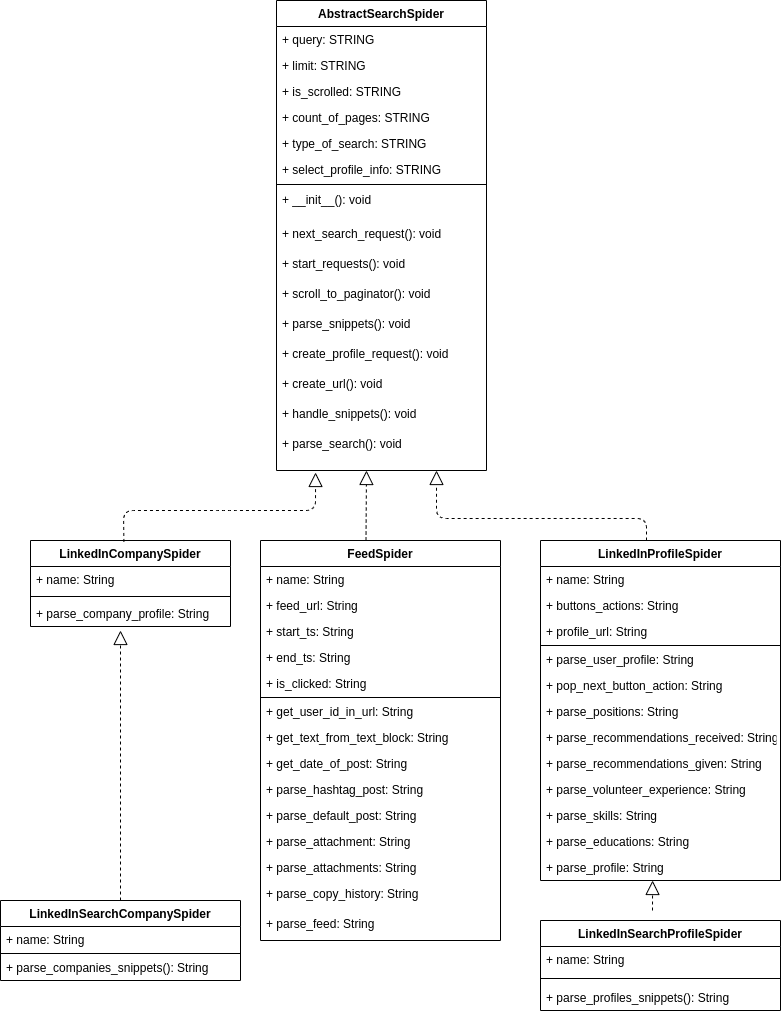
\includegraphics[height=14cm,keepaspectratio]{pictures/LinkedInWeb.png}}
        \caption{Диаграмма классов сборщик в социальной сети LinkedIn web.}
        \label{ris:image}
    \end{figure}
    \begin{itemize}
        \item AbstractSearchSpider -- абстрактный класс для поиска и сбора людей и организаций;
        \item LinkedInCompanySpider -- сборщик данных компаний;
        \item FeedSpider -- сбор данных новостной ленты пользователя; 
        \item LinkedInProfileSpider -- сборщик данных пользователей;
        \item LinkedInSearchCompanySpider -- поисковик компаний внутри социальной сети. При настройке имеет возможность 
        собирать информацию о найденных организациях;
        \item LinkedInSearchProfileSpider -- поисковик пользователей внутри социальной сети. При настройке имеет возможность
        собирать информацию о найденных людях.
    \end{itemize}
    \item поиск и сбор с помощью закрытого LinkedIn API:
    \begin{figure}[H]
        \center{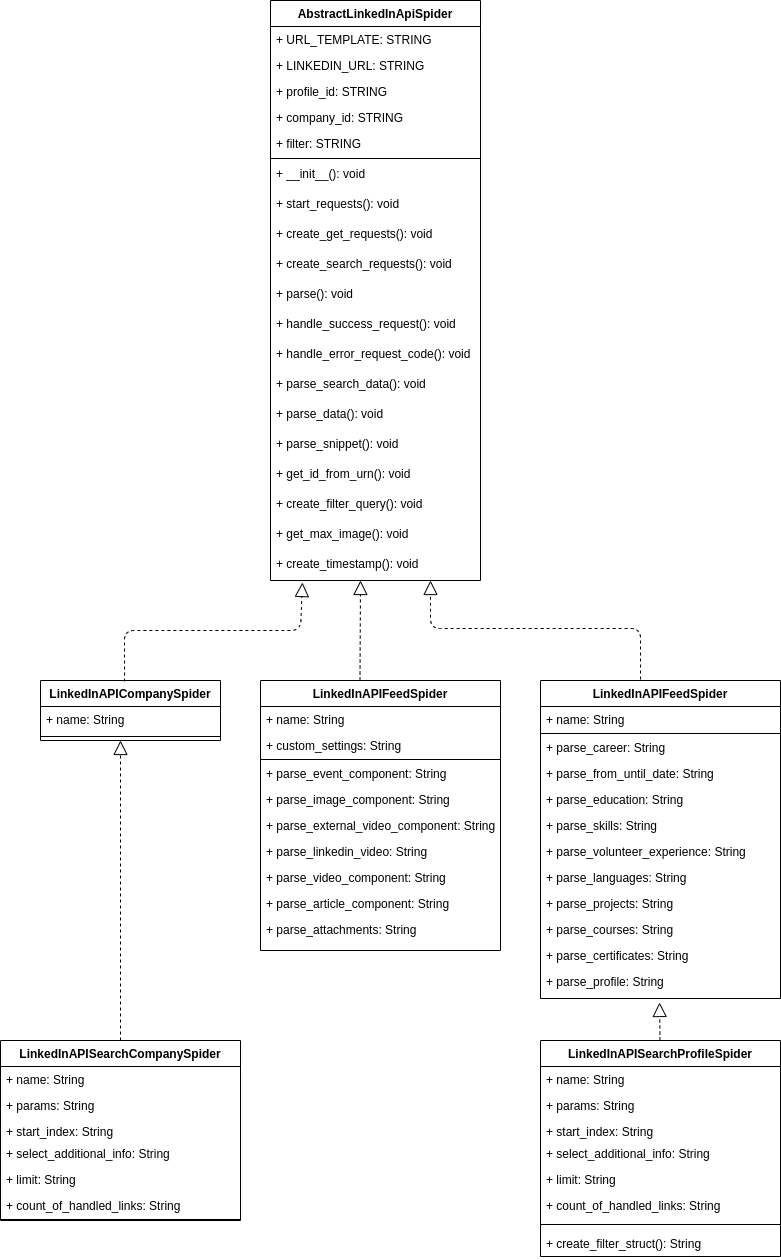
\includegraphics[height=14cm,keepaspectratio]{pictures/LinkedInAPI.png}}
        \caption{Диаграмма классов сборщик в социальной сети LinkedIn API.}
        \label{ris:image}
    \end{figure}
    \begin{itemize}
        \item AbstractLinkedInApiSpider -- класс, который эмулирует для получения данных из социальной сети посредством
        API;
        \item LinkedInAPICompanySpider -- сборщик данных заданной компании;
        \item LinkedInAPIFeedSpider -- сборщик новостной ленты;
        \item LinkedInAPIProfileSpider -- сборщик данных заданного пользователя;
        \item LinkedInAPISearchProfileSpider -- производит поиск пользователей по заданным фильтрам. Имеет возможность 
        собирать информацию о найденных людях при настройке;
        \item LinkedInAPISearchCompanySpider -- производит поиск компаний по заданным фильтрам. Имеет возможность 
        собирать информацию о найденных организациях при настройке.
    \end{itemize}
    \item Вспомогательные классы:
    \begin{itemize}
        \item AccountStatus -- перечисление со статусом аккаунта, под которым мы пытаемся собирать информацию в социальной
        сети;
        \item LinkedInCredentialsDownloaderMiddleware -- если в приложении нет cookie файлов или имеются устаревшие cookie, 
        данный класс перелогинивает указанный в настройках аккаунт при помощи GET и POST запросов в LinkedIn API. На выходе
        получаем обновленные cookie файлы и возможность дальше собирать информацию из социальной сети. 
    \end{itemize}  
\end{itemize} % Описание Экспериментальной части
\section{Заключение}
\label{sec:Chapter5} \index{Chapter5}
В данной работе были исследованы методы OSINT для поиска информации о человеке. Её решение было разбито на следующие задачи:
\begin{itemize}
    \item Поиск данных в поисковых сервисах:
    \begin{itemize}
        \item Провести анализ литературы и существующих решений для извлечения данных из поисковых систем;
        \item Разработать методы поиска и сбора информации из поисковых систем.
    \end{itemize}
    \itemПоиск данных в социальных сетях:
    \begin{itemize}
        \itemПровести анализ литературы и существующих решений для извлечения данных из социальных сетей;
        \itemРазработать методы поиска и сбора информации из социальных сетей.
    \end{itemize}
\end{itemize}

В рамках решения описанных выше задач были решены следующие:
\begin{itemize}
    \item проведен обзор литературы, статей, посвященных описанию различных OSINT-методов. Обзор показал, что методы поиска и 
    сбора могут отличаться, самые передовые приложения самостоятельно ищут, собирают и анализируют данные, представляю их 
    далее в виде дерева зависимостей;
    \item проведен обзор литературы, статей, связанных с устройством фреймворка Scrapy, Splash. Обзор показал, что на данный 
    момент использование Scrapy полностью оправдано, если необходимо производить сбор обширных данных на протяжении большого 
    количества времени, так и доказал, что использование Splash для рендера html-страниц полностью оправдано в нашей системе;
    \item Разработы методы поиска и сбора информации, собраны тестовые данные для оценки их качества;
    \item Проведена оценка качества с помощью сторонних метрик, которые отображают частоту вхождений каждого из полей.
\end{itemize}

По результату исследований разработаны и реализованы OSINT-методы поиска и сбора данных из поисковых источников и социальной сети
LinkedIn на языке Python.
\par
Данная работа может быть продолжена в следующих направлениях:
\begin{itemize}
    \item проведение исследований о возможности включения большего количества поисковых ресурсов и социальных сетей в систему;
    \item проведение исследований о возможности построения деревьев связи и наглядного отображения зависимостей в пользовательском
    интерфейсе.
\end{itemize}

Следует отметить, что разрабатываемое решение для LinkedIn осуществляет переходы только по URL-ссылкам, находящимся в атрибутах.
Но современные сайты могут использовать динамическую подгрузку данных, и на этот случай реализован рендер страницы при помощи 
Splash, а так же выявлен способ извелечения данных через API. Так что можно сделать вывод, что на данный момент система является
самодостаточной: она может обрабтывать статические, динамические сайты и вызовы через API. % Заключение

\nocite{*}
\bibliographystyle{gost71u} % Для соответствия требованиям об оформлении списка литературы
\bibliography{references}

% \section*{Приложение}
\addcontentsline{toc}{section}{Приложение}
\label{sec:Apendix} \index{Apendix}

 

\end{document}
